\chapter{Diskussion af resultater}

I dette kapitel vil der blive diskuteret relevante dele af de opnåede resultater og deres betydning for bachelorprojektet, samt hvilke muligheder og begrænsninger der er ved anvendelse af SRM. Til slut opsummeres der med den samlet vurdering af de opnåede resultater med relation til problemformuleringen.

\section{Konstant strøm}
Ud fra de forløbende tests, kom strømmen til at ændre sig. Ønsket var en konstant strøm på 283 $\mu A$. Problemet ved ikke at have en fast strøm gør, at det ikke bliver valide BI signaler, da denne faste strøm bruges til at udregne impedansen af BI signalet. Strømmen faldt til 104 $\mu A$, da elektroderne blev påmonteret måleobjektet, hvilket ikke stemmer overens med den beregnede/målte 283 $\mu A$. Da MyoWare Muscle Sensor blev tilføjet steg strømmen igen til 283 $\mu A$. Det kan skyldes det at MyoWare Muscle Sensor bruger en reference elektrode, som nu har fælles stel med BI måleren. Dette er ikke med i designet af BI måleren og derfor ikke tage høje for dette. Det kan være en mulig tilføjelse til BI måleren, da referance elektrode bliver brugt hvor man ønsker at måle BI signaler simultant med EMG signaler\cite{Nahrstaedt2012a}. 

\section{AA filter}
BI signalet afhænger af at AA filteret er korrekt bygget og fungere efter hensigten. Ellers vil den efterfølgende signalbehandling og visning af signalet være ubrugeligt pga. aliasering. Testene viser at AA filter fungerer efter hensigten ved at blive dæmpet ned til 95 dB ved 250 kHz. 

\section{Simultane målinger}
Ved at kunne foretage simultane målinger med BI og EMG signal, er hele essensen med at have disse to parametre. Dette gør at detektionen af et synk bliver mere valide, da der vil kunne konkluderes om det var et synk og ikke en anden bevægelse ved det pågældende tidspunkt. 



\section{Elektrode placering}
Ved brug af de store EKG elektroder, var der begrænset fleksibilitet mht. placeringen af disse elektroder. Inspirationen af placeringer af eletroderne blev fundet i flere artikler.\cite{Chester}
\cite{Schultheiss2013}. Forskellige placeringer af elektroder har indflydelse på det optaget BI signal\cite{Yamamoto2000}.  



\section{Digital signal behandling}
Da signalerne er samplet med en forholdsvis høj samplingrate på 500 kHz, giver det en stor mængde data. Med fordel kan denne store mængde være med til at det er muligt at signal behandle BI signal i det digitale domæne.
Behandlingen af envelope i det digitale domæne, gjorde at det nu ikke var nødvendigt med yderligere hardware komponenter, såsom ensretter og et lavpas filter.

\section{GUI}

Figur \ref{fig:synkfraGUI} og \ref{fig:synkfraArtikel} viser et synk, optaget med SRM og et fra en anden BI måler. Når disse to synk bliver stillet op imod hinianden ligner de meget godt hinanden. Både længden af synket og selve synkets bakkedal er sammenlignelige. Længden af synket kan i begge tilfældet aflæses til at vare ca. et sekund. Synkets bakkedal målt med SRM har også samme signatur. På dette grundlag er der argumenter for at det er muligt at detektere og vise et synk med SRM sammenlignet med en tilsvarende prototype BI måler.

\begin{figure}[H]
\centering
\begin{minipage}{.5\textwidth}
  \centering
  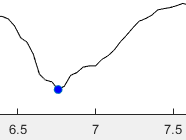
\includegraphics[width=.8\linewidth]{Figure/synkfraGUI}
  \captionof{figure}{Et synk målt med SRM. X aksen viser tid (s).}
  \label{fig:synkfraGUI}
\end{minipage}%
\begin{minipage}{.5\textwidth}
  \centering
  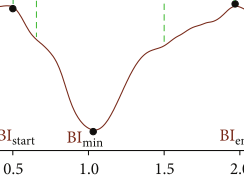
\includegraphics[width=.8\linewidth]{Figure/synkfraArtikel}
  \captionof{figure}{Et synk målt i en artikel\cite{Schultheiss2014}.X aksen viser tid (s).}
  \label{fig:synkfraArtikel}
\end{minipage}
\end{figure}

Variationen i et synk består af en ændring af impedansen på 5$\Omega$ \cite[s. 49]{Chester2014}. I figur \ref{Fig:synkfraGUI5ohm} kan et synk målt med SRM aflæses til at gå ned til ca. 5$\Omega$. Den målte ændring lægger sig fint og af hvad litteraturen oplyser. Ved en yderligere fintuning af den digitale signal behandling af BI signalet, ville man kunne få endnu bedre synk. Her er det parametrene såsom lavpas filter, downsample og smooth man ville kunne ændre på, for at for endnu bedre synk.

\begin{figure}[H]
\centering
{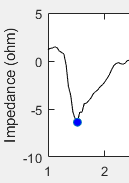
\includegraphics[width=4cm]
{Figure/synkfraGUI5ohm}}
\caption{Et synk målt med SRM, hvor synket er droppet til ca. 5$\Omega$. Dette er indenfor området for ændringen af synkets impedans.}
\label{Fig:synkfraGUI5ohm}
\end{figure} 

Algoritmen der finder peaks, altså i dette tilfælde synk, kan ses på figur \ref{Fig:synkfundet}. Disse synk illustrere med blå prikker. I Algoritimen er der sat en minimum størrelse for bakkedalen og afstanden i mellem hvert synk. Da dette er en meget forsimplet algoritme, vil der ikke blive fundet synk, hvis værdierne ikke er indenfor disse områder. Dette vil give en fejltælling af antal synk.

\begin{figure}[H]
\centering
{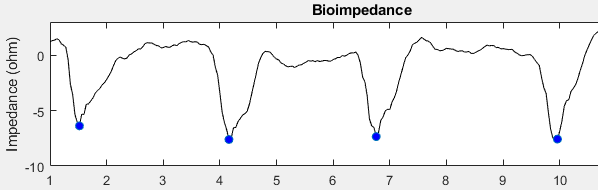
\includegraphics[width=\linewidth]
{Figure/synkfundet}}
\caption{Algoritmen der finder antal synk i en måling og informere sundhedspersonalet om antallet i GUI.}
\label{Fig:synkfundet}
\end{figure} 



\section{EMG måler}

På figur \ref{Fig:emgmaling} er EMG målingen vist. EMG måleren består af hardware der selv sørge for envelope og yderligere udglatning af EMG signalet. Da EMG signalet også er samplet ved 500 kHz giver det en mængde data man ønsker at reducere. Den nuværdende signalbehandling består i at downsample EMG signal og efterfølgende smooth. Dette er måske ikke nødvendigt, men disse parametre kan også justeres til man får det ønskede resultat. 

\begin{figure}[H]
\centering
{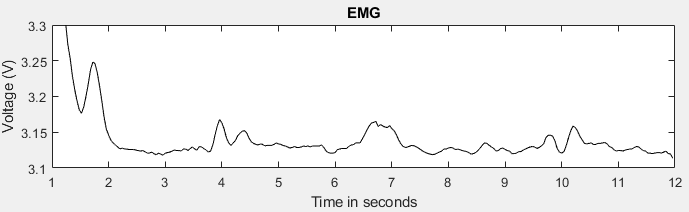
\includegraphics[width=\linewidth]
{Figure/emgmaling}}
\caption{En EMG måling med SRM. Her kan der aflæses fire udsving på EMG signalet.}
\label{Fig:emgmaling}
\end{figure} 

Det målte EMG signal kan sammenlignes med et EMG signal fra MyoWare Muscle Sensor's datablad \nameref{bilag15}. EMG signalet ser ud til at have samme peak, ved hvert EMG aktivitet. Udforingen med EMG måleren var, at optil det første sekund af en måling, genererede EMG måleren en høj peak. Hvilken kan muligvis relateres til når funktionsgeneratoren starter, når der foretages en måling. Dog påvirker det ikke resten af målingen.


\begin{figure}[H]
\centering
{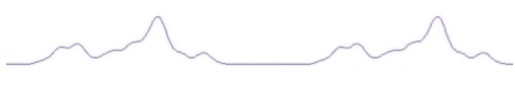
\includegraphics[width=\linewidth]
{Figure/emgsignal}}
\caption{Et eksampel på EMG signal fra MyoWare Muscle Sensor's datablad.}
\label{Fig:emgsignal}
\end{figure} 

Det færdige resultat af SRM kan ses på figur \ref{Fig:guiDone2}. Resultatet er simultane målinger af BI og EMG. I BI vises antal synk, som vises ude til venstre i GUI. Det er muligt at indskrive den akutelle strøm og vælge hvor langtid en måling skal foretages. Det er samtidig muligt at foretage de ønskede handlinger vha. de tre knapper. 

\begin{figure}[H]
\centering
{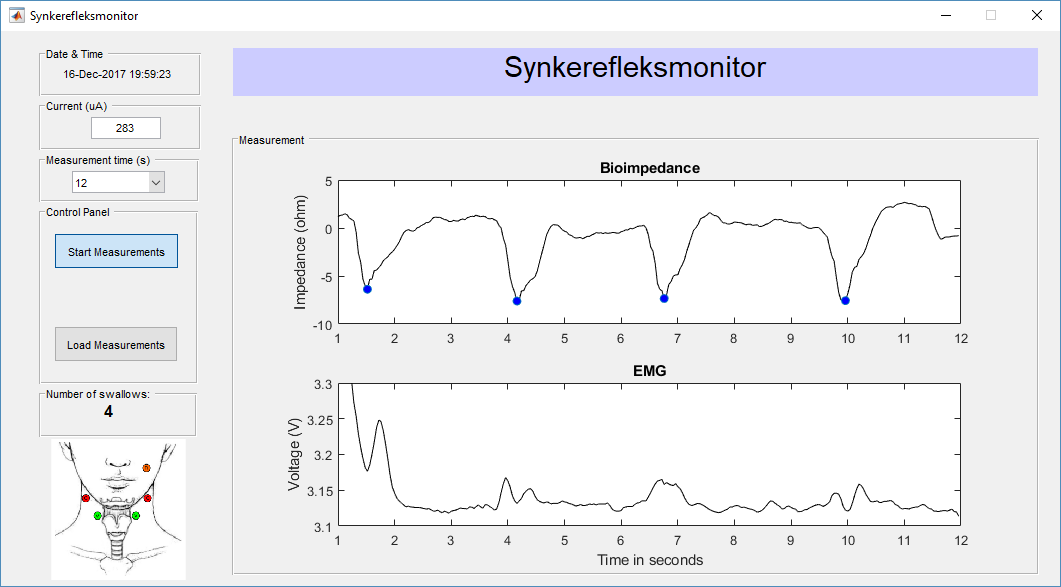
\includegraphics[width=\linewidth]
{Figure/guiDone}}
\caption{Det komplette interface af SRM.}
\label{Fig:guiDone2}
\end{figure} 



Den samlet vurdering af de opnåede resultater med relation til problemformuleringen kan opstilles i punktform. Disse punkter er samtidig resultater som vi er særlig stolte af. 

\begin{center}
\begin{large}
\begin{tabular}{|l l|}
\hline
-Udviklet funktionel Bioimpedansmåler&\checkmark \\[+2ex]
-Prisbillig i forhold til kommercielle BI målere & \checkmark \\[+2ex]
-SRM kan monitorere synkefrekvensen  & \checkmark \\[+2ex]
-SRM detektere synkefrekvensen & \checkmark \\[+2ex]
-Integreret kommerciel EMG måler & \checkmark \\[+2ex]
-Målingerne er simultane & \checkmark \\[+2ex]
-Brugergrænseflade til SRM  & \checkmark \\[+2ex]
-Ingen målinger fra personer med Dysfagi & $\div$ \\
\hline
\end{tabular}
\end{large}
\end{center}




